\documentclass[]{article}
\usepackage{indentfirst, graphicx}
\usepackage[margin=1in]{geometry}
\usepackage[T1]{fontenc}
\begin{document}

\title{APMA E4990 \\ Modeling Social Data \\ Final Project \\ Classifying arXiv.org Publications}
\author{Rasmi Elasmar}
\date{Friday, May 8, 2015}
\maketitle
\section*{Motivation}
ArXiv.org is a website that provides researchers with a place to publish and share academic papers with their peers. The papers are well-formatted with information about the authors and metadata that includes categorization of the paper into its field and any applicable sub-field. Papers come from a wide variety of categories, with astrophysics being among the most popular. This project focuses on using article summaries extracted from arXiv.org to classify astrophyiscs articles into their respective sub-categories, which would be a convenient feature when uploading and moderating new content.
\section*{Process}
Though most journals and sources for academic papers are often heavily restricted by access and copyright rules, arXiv provides a relatively open and simple API to pull article data from. ArXiv submissions have titles, one or more authors, summaries (abstracts), one or more categories, dates published, and revision details. A simple Python function was written to pull 2,000 articles for each of the six astrophysics subcategories and parse the data for each category into a local file. Articles per category were limited to the amount of the smallest category, which was 1600 for stellar astrophysics, leaving a total of 9,600 articles. The data for each category was then loaded into a single table with titles, summaries, authors, the first category in the list, the publication date, and the article ID. The selection of the first category as the defining one out of potentially multiple categories returned from the API would prove to be problematic for classification as discussed in later sections below. Data was then shuffled and split into 50/50 train/test set, with 4,800 articles in each set.
\section*{Classification}
The main method used for classification was a multinomial Naive Bayes classifier, as implemented in the scikit-learn Python package. Naive Bayes was chosen because of its simplicity and ability to handle multiple categories and large amounts of input, meaning it could work well for arXiv's massive database, and it would handle the train and test data quickly, which would allow for easy computation and fast iteration to try different approaches. Naive Bayes is also well-suited for text classification because of the generally independent nature of categorized text articles.
\subsubsection*{Naive Bayes}
The classic multinomial Naive Bayes approach consisted of parsing the article summaries into a sparse matrix that had rows for each article summary and columns for each word, with values representing word counts. This is a standard "bag of words" approach. This matrix is then used to train the MultinomialNB classifier, which can then be used to predict categories given test summaries.
\subsubsection*{With tf-idf}
Term frequency-inverse document frequency (tf-idf) is an alternate method of word counting that favors words that are more unique to each summary. Words that occur frequently in a summary are weighted less heavily, leaving more unique words with heavier weights. This matrix can then be used to train the MultinomialNB classifier in the same way the standard bag of words was.
\subsubsection*{With n-grams}
N-grams are a collection of consecutive words of size n, and incorporating n-grams into the counting process was simple. N-grams could potentially provide a better fit by taking into account phrases or words that occur together often, but they also present the issue of overfitting. For this test, n-grams of sizes $n=1,2,3$ were used.
\section*{Analysis}
The three approaches were accurate in classifying the articles into their correct categories approximately 80\% of the time, which is accurate enough to be useful, but not accurate enough to rely on without human intervention. In particular, pure Naive Bayes resulted in 81.10\% accuracy, including tf-idf yielded 81.29\% accuracy, and n-grams resulted in a slightly worse 79.92\% accuracy. Note that percentages change slightly between runs based on random shuffling and selection of training and test data, but the all the methods are generally with 1\% of each other, and they generally perform in the ranking similar to the one above. Tf-idf weighting likely resulted in a slight accuracy in increase due to the uniqueness of the terms used in the different subcategories of astrophysics, while n-grams likely resulted in a slight decrease in accuracy due to overfitting to phrases in the training set articles that weren't present in test set articles, but the effect does not seem to be significant over many runs.
\\
\centerline{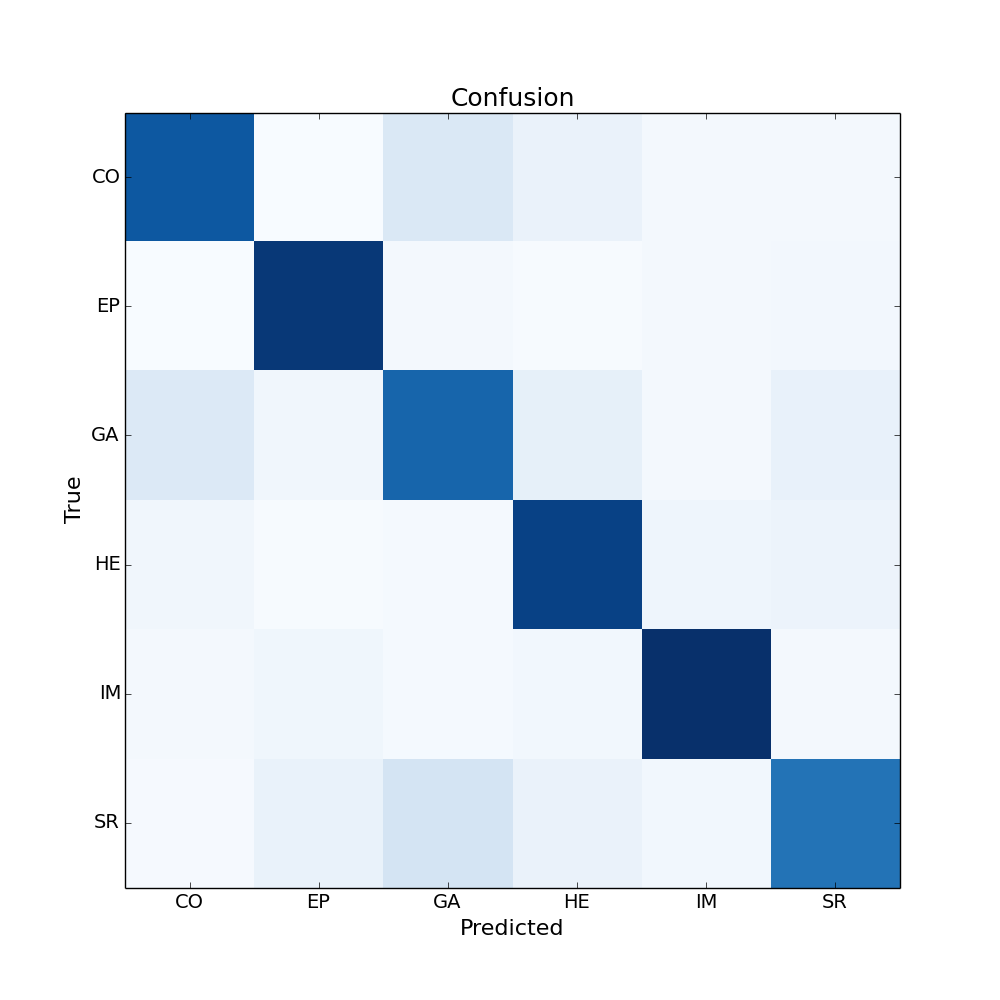
\includegraphics[width=210px]{confusion}}
\\
Investigating the confusion matrix gives great insight into what might have gone wrong with classification, and why Naive Bayes classification hit a ceiling around 80\% accuracy. When parsing the articles from arXiv, only the first category listing was chosen, potentially excluding multiple categories, which is a common occurrence for interdisciplinary research in astrophysics. The biggest sources of confusion in categorization were between Cosmology and Galaxies, and Galaxies and Stars. Both groups of subfields are intimately connected and it is to be expected that they share cross-categorized articles. This was not accounted for in my analysis, but potential approaches to accounting for this issue are presented in the next section.
\section*{Future Ideas}
There are many approaches that can be taken to improve this Naive Bayes classification or potentially classify articles using different methods entirely. 
To address the issue of cross-categorization, simply keeping track of all categories tagged to an article while training with some "main" category should suffice. It is not known if arXiv assigns a main category or just cross-lists articles with equal precedence across multiple categories. Regardless, training with one category and allowing for exceptions when the classifier suggests a second correct category should significantly increase classification accuracy.

It is not known if choosing a set number of articles (1600 in this case) for each category potentially created inaccuracies by over representing categories that are less popular than others. A possible solution to this is to simply select all articles submitted past a certain date and use all the results in whatever category distribution they present themselves in. Still, this might do more potential harm than good, since it may not cause inaccuracy to have more training data for underrepresented categories. Further testing is needed.

It may be worth using entirely different approaches to classification. SVMs are another popular approach to text classification and would be worth investigating. It would also be of interest to attempt classification based entirely on titles of articles. Alternatively, authors could be used to potentially graph networks of connections between authors, which could reveal the category of a paper based on closeness of connections to authors which are prominent in certain categories. Citations could add another layer of complexity and information to such a network.

Finally, it would be technically impressive, interesting, and useful to categorize papers across all subjects and subcategories available on the arXiv. Such a task would make great use of the massive arXiv archive. This could be done by first classifying by the main subject (astrophysics, computer science, math, statistics, etc.) then using a second layer of classification to group sub-categories within each subject. This would likely be an effective approach because the differences between larger subject areas would be more pronounced than differences between subcategories, and two layers of classifiers would be easier to build and manage than a single classifier which handled all possible subcategories across all subjects. To have such a classifier that could be trained and validated and updated with each submission based on human feedback (for example, whether a user manually adjusts a category after it is suggested by the algorithm) would be a fantastic application of machine learning. Such a classifier would be worth writing about, implementing, and submitting for production and publication in the arXiv.
\end{document}
